\documentclass[a4paper]{article}

\usepackage[ngerman]{babel}
\usepackage{dirtree}
\usepackage{underscore}
\usepackage{listings}
\usepackage{xcolor}
\usepackage{tabularx}
\usepackage{graphicx}
\usepackage{float}
\usepackage{subcaption}

\newenvironment{frage}[1]{%
	\par\noindent\textbf{Frage: #1}\par
}{\medskip}

\lstset{
	basicstyle=\ttfamily\small,
	backgroundcolor=\color{gray!10},
	frame=single,
	breaklines=true,
	xleftmargin=0pt,
	framexleftmargin=0pt,
	keywordstyle=\color{blue}\bfseries,
	commentstyle=\color{green!50!black},
	stringstyle=\color{orange},
	showstringspaces=false,
	}

\title{\textbf{Java Projekt DHBW SoSe 2025}}
\author{Elias Ciuman \\ Matrikel-Nr. 6265147}
\date{Abgabedatum: \today}

\begin{document}
	\maketitle
	\tableofcontents
	
	\newpage
	
	\section*{Projektdokumentation}
	
	
	\section{Einleitung}
	Im Rahmen des Moduls ``Programmieren'', das im ersten Studienjahr an der DHBW Mannheim im Studiengang "Angewandte Informatik" gelehrt wird, wurde innerhalb der Unit ``Programmieren in Java'' ein Programmentwurf gefordert.
	\\
	\\
	Dabei soll mithilfe der Google API eine Applikation entwickelt werden. Der Nutzer ist mit dieser in der Lage Google Kalender als iCalendar-Datei zu exportieren, um diese wiederum in einer beliebigen Kalender-App zu importieren. Die genauen Anforderungen werden im nächsten Abschnitt genauer erläutert.
	
	
	\section{Anforderungen}
	Im Folgenden werden die Anforderungen, welche gestellt wurden genau erläutert und in funktionale Anforderungen, sprich die tatsächlichen Funktionen, welche die Anwendung enthalten muss, unterteilt. Des Weiteren wird ein kurzer Blick auf die nicht-funktionalen Anforderungen geworfen, welche angeben, wie die Anwendung arbeiten soll.
	
	\subsection{Funktionale Anforderungen}
	Die vorliegende Aufgabenstellung wurde in zwei Teilaufgaben unterteilt:
	
	
	\subsubsection{Aufgabe 1)}
	Ziel der Aufgabe ist es ein Programm zu entwickeln, welches über einen Befehl innerhalb einer Konsole ausgeführt werden soll. Dabei ist vorgegeben die folgenden Argumente des Befehls abzugreifen, um als Ergebnis die geforderte iCal-Datei zu erhalten:
	\begin{itemize}
		\item Klassenname
		\item Start-Datum
		\item End-Datum
		\item Dateiname
	\end{itemize}
	
	
	\subsubsection{Aufgabe 2)}
	Im zweiten Teil soll eine Benutzeroberfläche zu der bestehenden Anwendung eingefügt werden.
	Die Startseite enthält die Tabelle mit den Namen der Ereignissen innerhalb des Kalenders, sowie den Start- und Endzeitpunkt. Der Nutzer soll außerdem die Möglichkeit besitzen aus drei Menüs mit jeweiligen Untermenüs auszuwählen:
	\pagebreak
	\begin{itemize}
		\item File
			\begin{itemize}
				\item Save - Speichert die iCal-Datei
				\item Exit - Beendet das Programm
			\end{itemize}
		\item Application
			\begin{itemize}
				\item Setting - Einstellungen, aus welchem Kalender von wann bis wann Events angezeigt werden
			\end{itemize}
		\item Help
			\begin{itemize}
				\item About - Zeigt Informationen über den Entwickler an
			\end{itemize}
	\end{itemize}
	Initial soll im Hauptfenster nur die Spaltenüberschriften ``Ereignis'', ``von'' und ``bis'' angezeigt werden. Nach dem die Einstellungen von dem Nutzer durchgeführt wurde, zeigt die Tabelle alle verfügbaren Ereignisse innerhalb des Zeitraums in der Tabelle an.
	Der Dialog ``Setting'' gibt dem Nutzer die Möglichkeit alle Einstellungen für den Export zu treffen. Dabei soll die Kalender-URL, sowie der Zeitraum von und bis eingetragen werden. Beim Klicken auf den Button ``OK'' werden die Einstellungen übernommen, bei ``Cancel'' wiederum sollen die Einstellungen verworfen werden, dennoch werden die vorherigen Einstellungen belassen.
	
	\subsection{Nicht-funktionale Anforderungen}
	Um die oben genannten Funktionen zu erreichen soll die Google API verwendet werden. Um dies zu erreichen sollen alle nötigen Bibliotheken sowie Gradle installiert werden. Gradle wird in dem dritten Abschnitt erläutert.
	Die Benutzeroberfläche soll mit einer Bibliothek bspw. Swing oder JavaFX erstellt werden. Es können optionale Features innerhalb des zweiten Aufgabenteils eingefügt werden.
	\begin{itemize}
		\item Input-Validierung
		\item Dateneingabe: JSpinner-Felder für Datumseingabe
		\item Speicherung von Einstellungen
	\end{itemize}
	
	
	\section{Projektarchitektur}
	Dieser Abschnitt handelt von dem grundlegenden Aufbau des gesamten Projekts und die verwendetet Technologien und Bibliotheken.
	
	\subsection{Verwendete Technologien}
	Um die Schnittstelle zwischen den Google-Diensten und dieser Applikation zu erreichen, wurde die \textbf{Google-Calendar-API} verwendet.
	Das Build- und Abhängigkeitsmanagement übernimmt \textbf{Gradle}. Für die Erstellung und Darstellung der Benutzeroberfläche kommt \textbf{Java Swing} zum Einsatz.
	
	\subsection{Projektstruktur}
	Innerhalb des \textbf{src-Ordners} befindet sich der für diesen Projektentwurf relevanter Quellcode. Dabei wurde darauf geachtet eine klare Struktur der Java-Klassen zu erreichen. So befinden sich innerhalb des \textbf{Swing-Ordners} alle Klassen für Swing-Komponenten, welche verwendet wurden.
	\\
	\dirtree{%
		.1 JavaProject_Ciuman_Elias/.
		.2 build/.
		.2 doc/.
		.2 gradle/.
		.2 src/.
		.3 main/.
		.4 java/.
		.5 calendar/.
		.5 main/.
		.5 swing/.
		.5 util/.
		.4 resources/.
		.2 tokens/.
		.2 build.gradle.
		.2 gradlew.
		.2 gradlew.bat.
		.2 README.md.
		.2 settings.gradle.		
	}
	
	\section{Implementierung}
	Dieser Abschnitt befasst sich mit der eigentlichen Bearbeitung und Implementierung der oben genannten Aufgaben.
	
	\subsection{Aufgabe 1)}
	\textbf{Relevante Klassen:} clsGoogleCalendarService, clsCalenderExporter, clsMain  
	\\
	\\
	\textbf{clsGoogleCalendarService} Zunächst werden die nötigen Konstanten erstellt, welche für die Initialisierung des Projekts verwendet werden. Darunter fallen Dinge wie der Name der Anwendung, welche zuvor innerhalb der Google-Projekte selbst erstellt wurde, sowie Konstanten zur Verarbeitung der JSON-Datei, welche für die Authentifizierung benötigt wird.
	Dem folgen drei Methoden:
	\begin{description}
		
		\item[\texttt{getCredentials()}] Diese Methode ermöglicht es, dass dieses Programm auf den Google-Kalender zugreifen kann. Dafür liest diese die Daten aus der credentials.json aus um diese in der Autorisierung mit Hilfe von OAuth2 zu verwenden. Außerdem wird ein lokaler Speicher für die Tokens erstellt, um diese verwenden zu können. Danach wird ein lokaler Webserver gestartet, um den OAuth2-Callback von Google zu empfangen, welcher der User im Browser akzeptieren muss, um das Programm verwenden zu können.
		
		\item[\texttt{getCalendarService()}] Die einzige Aufgabe dieser Methode ist es einen authentifizierten Google-Calendar-Service aufzubauen, um auf diesen zuzugreifen zu können. Dafür wird die \texttt{getCredentials()}-Methode verwendet, um die Authentifizierung durchzuführen.
		
		\item[\texttt{getEvents()}] Diese Methode holt alle verfügbaren Events aus der übergebenen Kalender-ID, sowie dem Zeitraum. Dafür wird zunächst der Google-Calendar-Service aufgerufen und der Start- sowie Endzeitpunkt in einer Variable gespeichert.
		Danach wird eine Abfrage an die Google-Calendar-API gesendet, welche alle Events mit den jeweiligen übergebenen Parametern abruft. Diese Events werden in einer Map, also in Schlüssel-Wert-Paaren geschrieben. Diese Liste wird zurückgeben per \texttt{return}-Statement
	\end{description}
	
	\textbf{clsCalendarExporter} Diese Klassen beinhaltet lediglich die \texttt{export()}-Methode, welche mit einer Map von Events sowie dem Namen der zu erstellenden Datei aufgerufen wird. Diese iterierter durch jeden Eintrage dieser Liste und schreib diese in eine Datei.
	\\
	\\
	\textbf{clsMain} Innerhalb der Main-Klasse werden die oben genannten Klassen eingebunden, sowie die Argumente, welche über die Konsole den Nutzer eingegeben werden verarbeitet und in Variablen gespeichert. Demnach wird zunächst ein Google-Calendar-Service-Objekt erstellt und die \texttt{getEvents()}-Methode aufgerufen. Die Events werden in einer Liste gespeichert, welche, nachdem das CalendarExporter-Objekt erstellt wurde, der \texttt{export()}-Methode übergeben wird. Nach erfolgreicher Ausführung erhält der Nutzer seine Datei standardmäßig in das Projektverzeichnis abgelegt.
	
	\subsection{Aufgabe 2)}
	\textbf{Relevante Klassen:} DateLabelFormatter, dlgAbout, dlgSettings, MainFrame, clsGoogleCalendarUtil, clsMain
	\\
	\\
	Dieser Aufgabenteil handelt von der Implementierung einer Benutzeroberfläche. Dafür wurde Swing verwendet. Die folgende Auflistung erklärt die jeweiligen Klassen und deren Funktion:
	\begin{description}
		
		\item[\texttt{MainFrame}] Hierbei handelt es sich um das Hauptfenster der Anwendung, welches der Nutzer bei Starten der Anwendung zuerst sieht. Dieses erbt von dem JFrame und nutzt als Layoutmanger das BorderLayout. Initial ist eine leere JTable mit den Spaltenüberschriften zusehen. Genaueres dazu findet sich in den Fragen zu Aufgabe 2) im sechsten Abschnitt dieser Dokumentation. Nachdem der User die Einstellungen getroffen hat, wird über eine for-Schleife die Zeilen dynamisch in die Tabelle eingefügt. Außerdem findet sich in dem Hauptfenster die Menüleiste, welche mit einer JMenuBar realisiert wurde. Die einzelnen Menüpunkte werden mit JMenuItems eingebaut. Des Weiteren beinhaltet diese Klasse die Realisierung der Menüpunkte durch ActionListener, welche auf einen Klick des Nutzers reagieren und die entsprechende Aktion ausführen. Beispielsweise für den Export wird dafür auf die zuvor definierten Klassen \texttt{clsGoogleCalendarService} und \texttt{clsCalendarExporter} sowie deren Methoden zurückgegriffen.
		
		\item[\texttt{dlgAbout}] Dieser Dialog wird angezeigt, wenn der Nutzer im Menü auf Help/About klickt. Dieser enthält Informationen zum Entwickler sowie die optionalen Features, welche diese Anwendung enthält. Diese Klasse erbt von JDialog und ist ein modaler Dialog, welcher über dem Hauptfenster angezeigt wird und verwendet ein BorderLayout um den Inhalt zentriert anzuzeigen. Der Inhalt wird durch ein JLabel mit HTML-formatiertem Text angezeigt. Die Schriftgröße passt sich automatisch an die Fenstergröße an.
		
		\item[\texttt{dlgSettings}] Hier kann der Nutzer die Einstellungen treffen, um die Events im Hauptfenster anzeigen zu können. Diese Klasse erbt von JDialog und ist ein Modal-Dialog, welcher über den Hauptfenster angezeigt wird. Für das Layout wurde ein BorderLayout, für das Formular selbst ein GridLayout verwendet. Diese Klasse enthält zwei Textfelder für die Kalender-ID und den Namen der Datei, nachdem der Export durchgeführt wurde. Die Dateiendung .ics muss nicht vom Nutzer eingegeben werden, diese wird automatisch von der Anwendung angehängt. Für die Realisierung der Datumsfelder wurde ein externes Repository verwendet (JDatePickerImpl) um dem Nutzer eine benutzerfreundlichen Datepicker bereitzustellen sowie eine damit einhergehende Input-Validierung. Außerdem befinden sich in diesem Dialog zwei JButtons ´´OK'' und ``Cancel''. Diese Buttons besitzen jeweils einen ActionListener. Der OK-Button führt eine Input-Validierung aus. Dafür wird zunächst überprüft, ob der Nutzer jedes Feld ausgefüllt hat. Ansonsten wird eine Fehlermeldung angezeigt. Außerdem wird überprüft, ob das Von-Datum vor dem Bis-Datum liegt. Danach wird die Kalender-ID asynchron überprüft, ob diese gültig ist. Dafür wird ein Loading-Dialog angezeigt, während die Anwendung die ID überprüft. Dafür wird im Hintergrund eine Util-Klasse aufgerufen \texttt{clsGoogleCalenderUtils}. Diese überprüft mit der Methode \texttt{calendarIdExists(Calendar calendarService, String calendarId)} ob bei einem Aufruf der Kalender-ID ein Fehler mit dem Code 404, sprich der Kalender wurde nicht gefunden, auftritt. Wenn dies passiert, bekommt der Nutzer eine Fehlermeldung, ansonsten wird das Programm ausgeführt und der Nutzer erhält die Tabelle mit den Events.
		
		\item[\texttt{DateLabelFormatter}] Diese "Hilfsklasse" wird verwendet für die Anzeige und Eingabe von Datumswerten in JDatePicker. Hier werden Strings in Values sowie Values in Strings umgewandelt. Values werden für die Verarbeitung benötigt, Strings für die Anzeige
	\end{description}
	
	\subsection{Speicherung von Daten}
	\textbf{Relevante Klassen:} dlgSettings, clsSettingsManager
	\\
	\\
	Um die Speicherung von eingegebenen Daten auch nach dem Schließen der Anwendung zu realisieren wurde die Klasse \texttt{clsSettingsManager} erstellt. Dabei werden die Daten in der \texttt{settings.properties} innerhalb des Projektverzeichnisses gespeichert. Diese Klasse enthält zwei Methoden. \textbf{loadSettings()} versucht bei der Erstellung des clsSettingsManager-Objekts diese Datei zu laden. \textbf{saveSettings()} wird von der der dlgSettings-Klasse aufgerufen, nachdem der Nutzer seine Daten eingegeben hat und auf \texttt{OK} klickt. Die Daten werden in der zuvor genannten Datei gespeichert, sodass diese erhalten bleiben, auch wenn die Anwendung geschlossen wird.
	 
	
	
	\section{Benutzung}
	\subsection{Installation und Voraussetzung}
	Da dieses Projekt in eine .jar-Datei gebaut wurde, muss für die Verwendung der Anwendung lediglich Java (mindestens JRE) auf dem Computer installiert sein.
	Zum Beispiel:
	\begin{itemize}
		\item https://openjdk.org/
		\item https://www.oracle.com/de/java/
		\item ...
	\end{itemize}
	Außerdem muss das Projektverzeichnis (über Moodle hochgeladen) heruntergeladen und an einen beliebigen Ort entpackt werden.
	Es wird die credentials.json mitgeliefert. Dort ist ein Test-Google-Account angelegt, welcher einen Primary-Kalender enthält (für den Konsolen-Aufruf) sowie ein Kalender, welcher mit einer ID aufgerufen werden kann.
	
	\subsection{Bedienungsanleitung}
	
	Beide Aufgabenteile können mit diesem Projekt ausgeführt werden
	
	\subsubsection*{Export per Argumenten in der Konsole}
	\begin{enumerate}
		\item Konsole (cmd) öffnen
		\item Zum Projektverzeichnis mit \texttt{cd} navigieren
		\item Anwendung mit dem Befehl \texttt{java -cp build/libs/JavaProject_Ciuman\\_Elias-1.0.jar main.clsMain <Start-Datum> <End-Datum> <Dateiname>.ics} aufrufen
		\item Dabei das folge Datums-Format verwenden: YYYY-MM-DD
		\item Beispiel: \texttt{java -cp build/libs/JavaProject_Ciuman_Elias-1.0.jar main.clsMain 2025-07-01 2025-12-31 calendar.ics}
		\item Die Datei wird in das Projektverzeichnis abgelegt
	\end{enumerate}
	
	\subsubsection*{Export per GUI}
	\begin{enumerate}
		\item Konsole (cmd) öffnen
		\item Zum Projektverzeichnis mit \texttt{cd} navigieren
		\item Die GUI öffnet sich mit dem Befehl \texttt{java -cp build/libs/JavaProject\\_Ciuman_Elias-1.0.jar main.clsMain}
		\item Es erscheint das Hauptfenster mit leerer Tabelle
		\item Um Einstellungen zu treffen in der Menüleiste auf \textbf{Appliaction} dann \textbf{Settings}
		\item Es öffnet sich ein Modalfenster mit den Einstellungen
		\item Dort in das Feld \textbf{Kalender-ID} folgende ID eintragen: \\ \texttt{aaed8773fd1b77d61ddbc771aa99a3da048c9ee90107\\9dd8afb3dfa389417c5c@group.calendar.google.com}\\
		\texttt Die anderen Felder nach Belieben ausfüllen. Es sind Ereignisse im Kalender vom 1.7.25 bis 31.12.25 eingetragen
		\item Es wird überprüft, ob der Kalender existiert. Hier kann in der Kalender-ID auf \texttt{primary} eingegeben werden, sollte es zu Fehlern kommen
		\item Mit OK die Einstellungen bestätigen
		\item Die Tabelle ist jetzt mit den Events je nach Eingabe befüllt
		\item Über das Menü \textbf{File} dann \textbf{Save} wird die Datei in das Download-Verzeichnis des Nutzers gespeichert
	\end{enumerate}
	
	\section{Fragen}
	In diesem Abschnitt werden die gestellten Fragen zu den jeweiligen Aufgaben beantwortet.
	
	\subsection{Fragen zu Aufgabe 1}
	
	\begin{frage}{Welche Funktion bietet das Tool Gradle? Wofür kann es eingesetzt werden?}
	 Gradle ist ein sogenannten "Build-Automatisierungs-Tool" unter anderem für Java-Projekte wie dieses. Die Aufgaben, welches dieses Tool übernimmt sind die Kompilierung, Testdurchführungen, Archivierung sowie Deployments auf Basis einer programmierbaren DSL (Groovy oder Kotlin). Gradle wird verwendet um größere Projekte effizient zu bauen. Ein weiterer Vorteil ist die Unterstützung Plugins für Java zu integrieren.
	\end{frage}
	\\
	\begin{frage}{Was bedeuten die Schritte ``API aktivieren'' und ``OAuth-Zustimmungsbildschirm konfigurieren''?}
		
		\textbf{API aktivieren} bedeutet, dass das vorhandene Projekt Dienste der sogenannten Schnittstelle verwenden kann. In diesem Beispiel wird die Google-Calendar-API verwendet. Es muss sichergestellt werden, dass die API aktiviert wurde, um die vorhandenen Dienste und Services dieser API in diesem Projekt verwenden zu können.
		
		\textbf{OAuth-Zustimmungsbildschirm konfigurieren} wird benötigt, damit der Nutzer diesen Bildschirm zu sehen bekommt, wenn er die Anwendung aufruft, um seine Zustimmung zu geben, dass die die Google-Calendar-API gewisse Daten zum Ausführen der Anwendung verwenden darf. Dafür muss der Ersteller dieser Anwendung zuvor diesen Zustimmungsbildschirm konfigurieren mit unter anderem dem Anwendungsname oder der Support-E-Mail sowie die angeforderten Zugriffsrechte (Scopes). 
	\end{frage}
	
	\begin{frage}{Wie kann man in einer IDE die Google Calendar API verfügbar machen, so dass diese für ein Projekt verwendet werden kann?}
		
		Im ersten Schritt muss innerhalb der Google-Cloud ein Projekt erstellt werden und die Google-Calendar-API aktiviert werden. Des Weiteren ist es nötig die OAuth zu aktivieren und die credentials.json herunterzuladen und im Projektverzeichnis unter dem resources-Ordner im src-Ordner zu speichern. Danach muss man die Google Calendar-Client Bibliothek in das Projekt einbinden. In diesem Fall wird Gradle verwendet. Folgender Code-Abschnitt wird dafür in die gradle.build eingefügt werden.
		\begin{lstlisting}[language=]
implementation 'com.google.apis:google-api-services-calendar:v3-rev20230808-2.0.0'
implementation 'com.google.api-client:google-api-client:2.2.0'
implementation 'com.google.oauth-client:google-oauth-client-jetty:1.34.1'	
		\end{lstlisting}
	\end{frage}


	\begin{frage}{Erläutern Sie die Code-Zeilen final NetHttpTransport HTTP TRANSPORT
			= GoogleNetHttpTransport.newTrustedTransport(); Calendar service
			= new Calendar.Builder(HTTP TRANSPORT, JSON FACTORY, getCredentials(HTTP TRANSPORT))
			.setApplicationName(APPLICATION NAME) .build();}
		Diese Code-Zeilen erstellen einen Calendar-Service um auf den Google-Kalender in der Anwendung zugreifen zu können. Dafür wird zunächst die Transport-Schicht für HTTP-Anfragen erstellt. Dafür wird ein Objekt erzeugt, mit SSL-Zertifikaten, sodass HTTPS verwendet werden kann. Das Schlüsselwort final bedeutet, dass HTTP_TRANSPORT im weiteren Verlauf des Programms nicht mehr verändert werden kann.
		Danach wird ein Calendar-Objekt erstellt. Calendar.Builder() erstellt einen Builder für den Google Calendar Service. Dabei erhält dieser die folgenden Parameter:
		\begin{itemize}
			\item HTTP_TRANSPORT - zuvor erstellte HTTPS-Verbindung
			\item JSON_FACTORY - JSON-Verarbeitungsobjekt, konvertiert Daten zwischen Java-Objekten und JSON.
			\item getCredentials(HTTP_TRANSPORT) - Authentifizierungsdaten (OAuth 2.0 Credentials), damit API auf gegebenen Google-Account zugreifen darf.
		\end{itemize}
		\texttt{.setApplicationName(APPLICATION_NAME)} setzt den Namen der Anwendung aus der Variable APPLICATION_NAME und \texttt{.build()} baut final das Calendar-Service-Objekt, um diesen dann für die weitere Logik der Anwendung zu verwenden.
	\end{frage}
	
	\subsection{Fragen zu Aufgabe 2}
	
	\begin{frage}{Wie definiert man Zeilen/Spalten für ein JTable-Objekt?}
		Dafür definiert man zunächst ein TableModel. Die Spalten werden durch ein String-Array beim Erstellen dieses TableModels angegeben \begin{lstlisting}[language=Java]
String[] columns = {"Ereignis", "von", "bis"};
		\end{lstlisting} Dieses Array wird dem TableModel übergeben. Zeilen werden dem Model mit \texttt{addRow()} hinzugefügt. Dabei werden innerhalb der runden Klammern die Daten der jeweiligen Spalten in der Zeile angegeben.
	\end{frage}
	\\
	\begin{frage}{Was muss beachtet werden, wenn bei einem JTable die Spaltenüberschriften angezeigt werden sollen}
		Dafür ist es nötig, die JTable innerhalb eines JScrollPane einzufügen. Das JScrollPane sorgt dafür, dass die Spaltenüberschriften sichtbar werden (JTableHeader).
	\end{frage}
	\\
	\begin{frage}{Welche Layoutmanager haben Sie für welchen Dialog/welches Fenster verwendet? Begründen Sie.} 
		\begin{tabularx}{\textwidth}{|l|l|X|}
			\hline
			\textbf{Dialog/Fenster} & \textbf{Layoutmanager} & \textbf{Begründung} \\
			\hline
			Mainframe/headerPanel & BorderLayout/BoxLayout & BorderLayout ist gut, um Hauptbereiche klar zu strukturieren / BoxLayout sorgt für saubere vertikale Ausrichtung der Überschriften \\
			\hline
			dlgSettings & GridLayout & GridLayout ist ideal für gleichmäßig verteilte Formularelemente \\
			\hline
			dlgAbout & BorderLayout & BorderLayout ermöglicht eine einfache Zentrierung des Inhalts im Dialog \\
			\hline
		\end{tabularx}
	\end{frage}
	\\
	\begin{frage}{Wie definiert man, welche Aktion bei der Auswahl eines Menüs ausgeführt werden soll?}
		Um die richtigen Aktionen bei der Auswahl eines Menüpunkts auszuführen werden \textbf{ActionListener} verwendet. Dem Listener wird die gewünschte Aktion übergeben und mit \texttt{addActionListener} mit dem dazugehörigen JMenuItem verbunden. 
		\begin{lstlisting}[language=java]
JMenuItem saveItem = new JMenuItem("Save");
saveItem.addActionListener(e -> {
	// Hier steht die Aktion, die beim Klicken auf Save ausgefuehrt werden soll
});
		\end{lstlisting}
		
	\end{frage}
	
	\section{Anhang}
	\appendix
	
	\subsection*{Screenshots aus der Anwendung}
	\begin{figure}[H]
		\centering
		
		\begin{subfigure}[t]{0.45\textwidth}
			\centering
			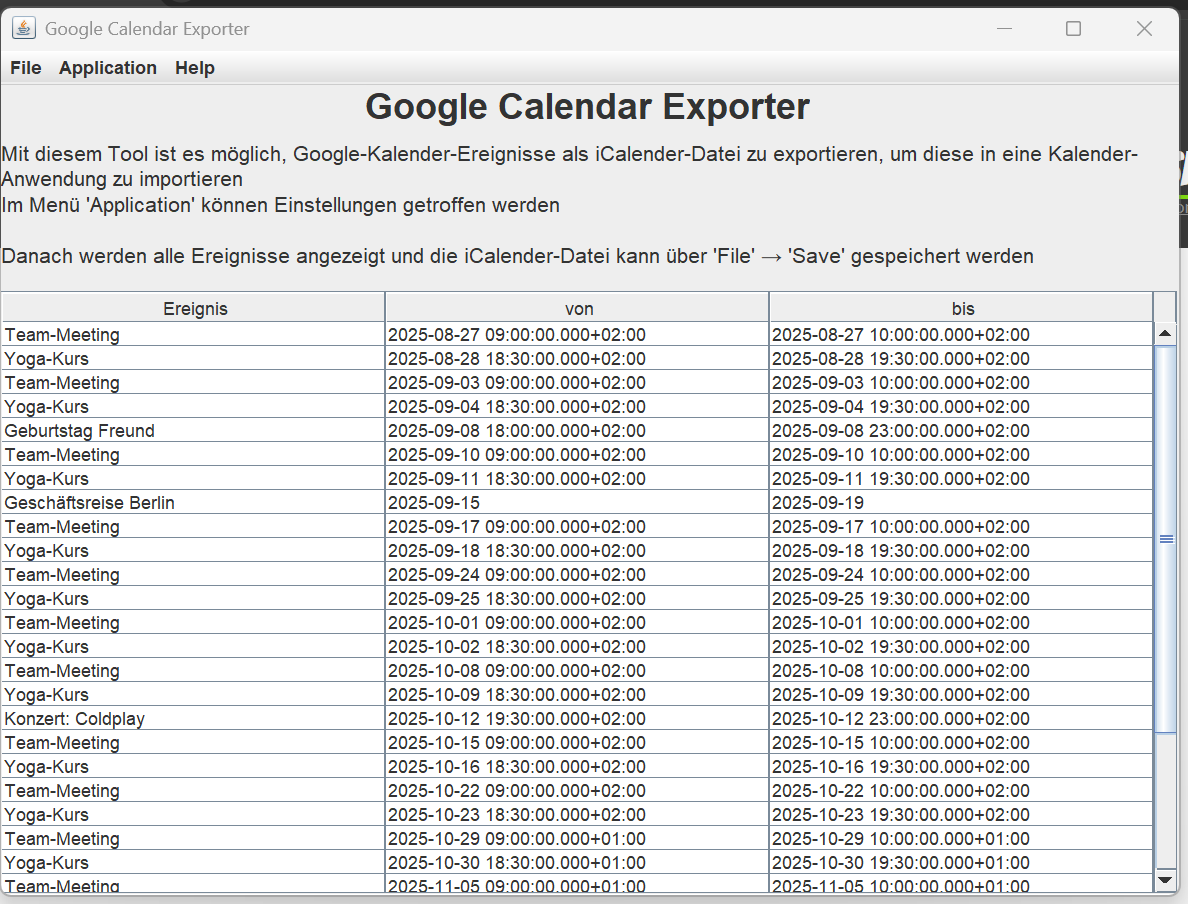
\includegraphics[width=\textwidth]{img/example_table.png}
			\caption{Tabelle mit Events}
		\end{subfigure}
		
		\vspace{1em}
		
		
		\begin{subfigure}[t]{0.45\textwidth}
			\centering
			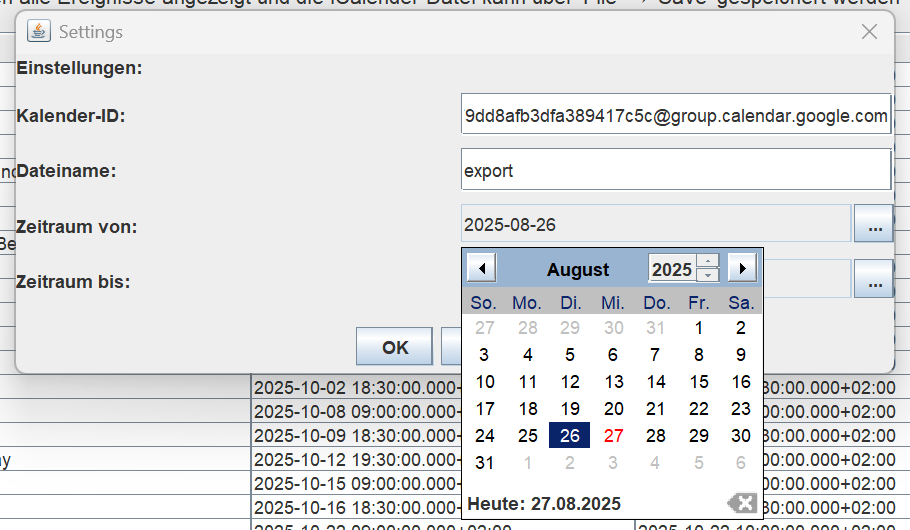
\includegraphics[width=\textwidth]{img/settings.png}
			\caption{Einstellungen}
		\end{subfigure}
		
		\vspace{1em}
		
		
		\begin{subfigure}[t]{0.45\textwidth}
			\centering
			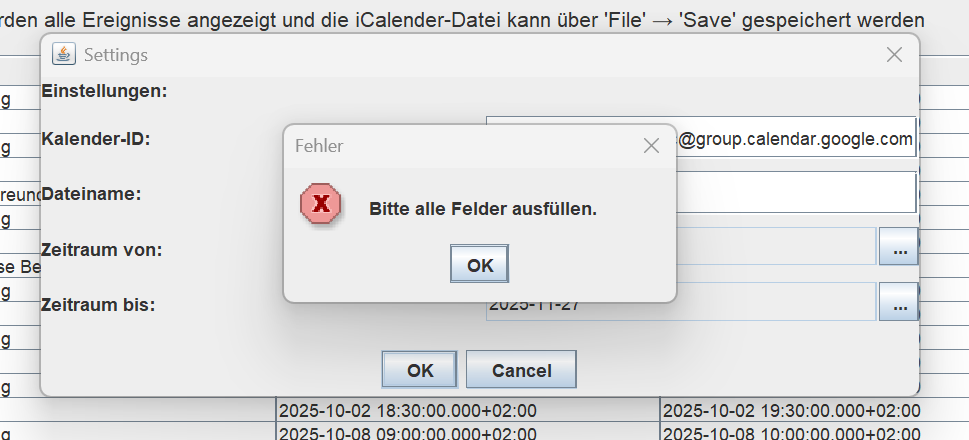
\includegraphics[width=\textwidth]{img/error_example.png}
			\caption{Fehlermeldung wenn nicht alle Felder ausgefüllt}
		\end{subfigure}
		
		\vspace{1em}
		
		
		\begin{subfigure}[t]{0.45\textwidth}
			\centering
			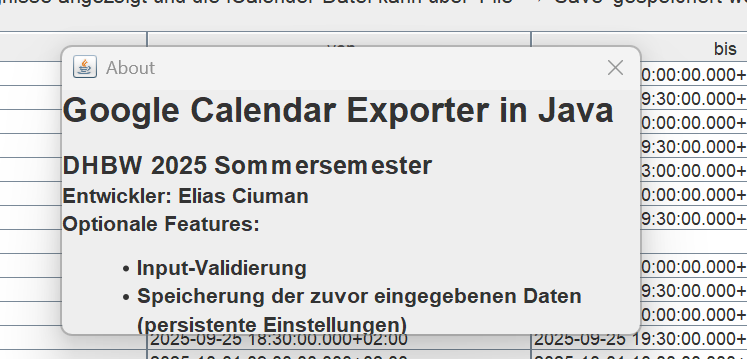
\includegraphics[width=\textwidth]{img/about_dialog.png}
			\caption{About-Dialog}
		\end{subfigure}	
		\caption{Screenshots aus der Anwendung}	
	\end{figure}
	
	\subsection*{Klassendiagramm für Aufgabe 1}
	
	\begin{figure}[H]
		\centering
		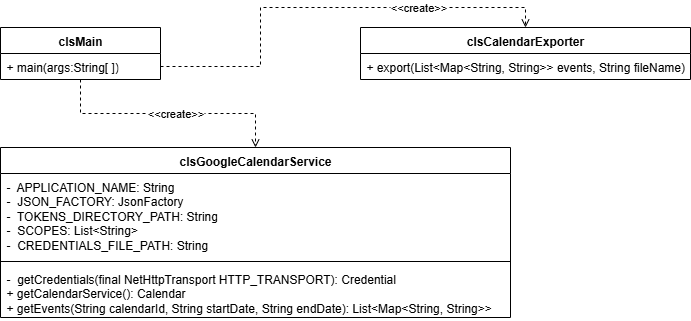
\includegraphics[width=\textwidth]{img/Klassendiagramm_Aufgabe1.png}
		\caption{Klassendiagramm Aufgabe 1}
	\end{figure}
	
	\subsection*{Aktivitätsdiagramm Export}
	\begin{figure}[H]
		\centering
		\includegraphics[width=\textwidth]{img/Aktivitätsdiagramm_Swing.png}
		\caption{Aktivitätsdiagramm Export}
	\end{figure}
	
\end{document}